% Jason Wang

A two-input NAND circuit is constructed on the bread board using the CD4007 gate array.

\FloatBarrier

\begin{figure}[h!]
	\centering
	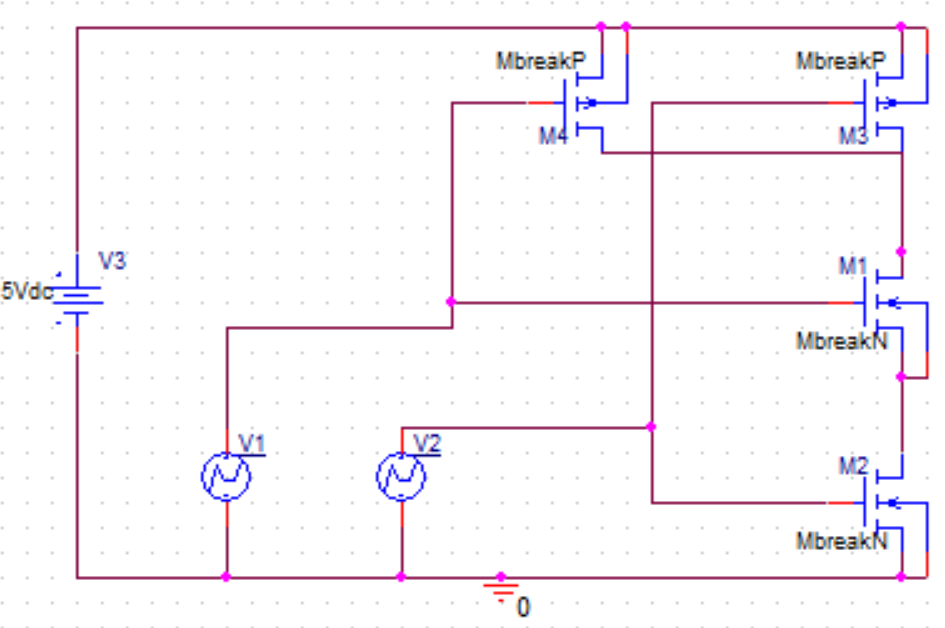
\includegraphics[scale=0.50]{../images/nand_schematic.PNG}
	\caption{Layout of Two-input NAND Gate}
	\label{fig:nand_schematic}
\end{figure}

\FloatBarrier

The two-input NAND gate has following logic chart (or truth table) where $x$ and $y$ are inputs and $S$ is the output and $0$ corresponds to low and $1$ corresponds to high.
The output voltage is taken at the drain node of the NMOS M1 in Figure \ref{fig:nand_schematic}.

\FloatBarrier

\begin{table}[h!]
	\centering
	\caption{Logic Chart of Two-input NAND Gate}
	\label{tab:logic_nand}
	\csvautotabular{../data/logic_nand.csv}
\end{table}

\FloatBarrier

The behavior of the NAND gate circuit is not tested using the oscilloscope due to complications in its construction on the bread board.
However, the behavior of the circuit is expected to be consistent with Figure \ref{\tab:logic_nand} where $0$ and $1$ correspond to low and high output voltages, respectively.
The following SPICE simulation shows the expected behavior of the NAND gate circuit.

\FloatBarrier

\begin{figure}[h!]
	\centering
	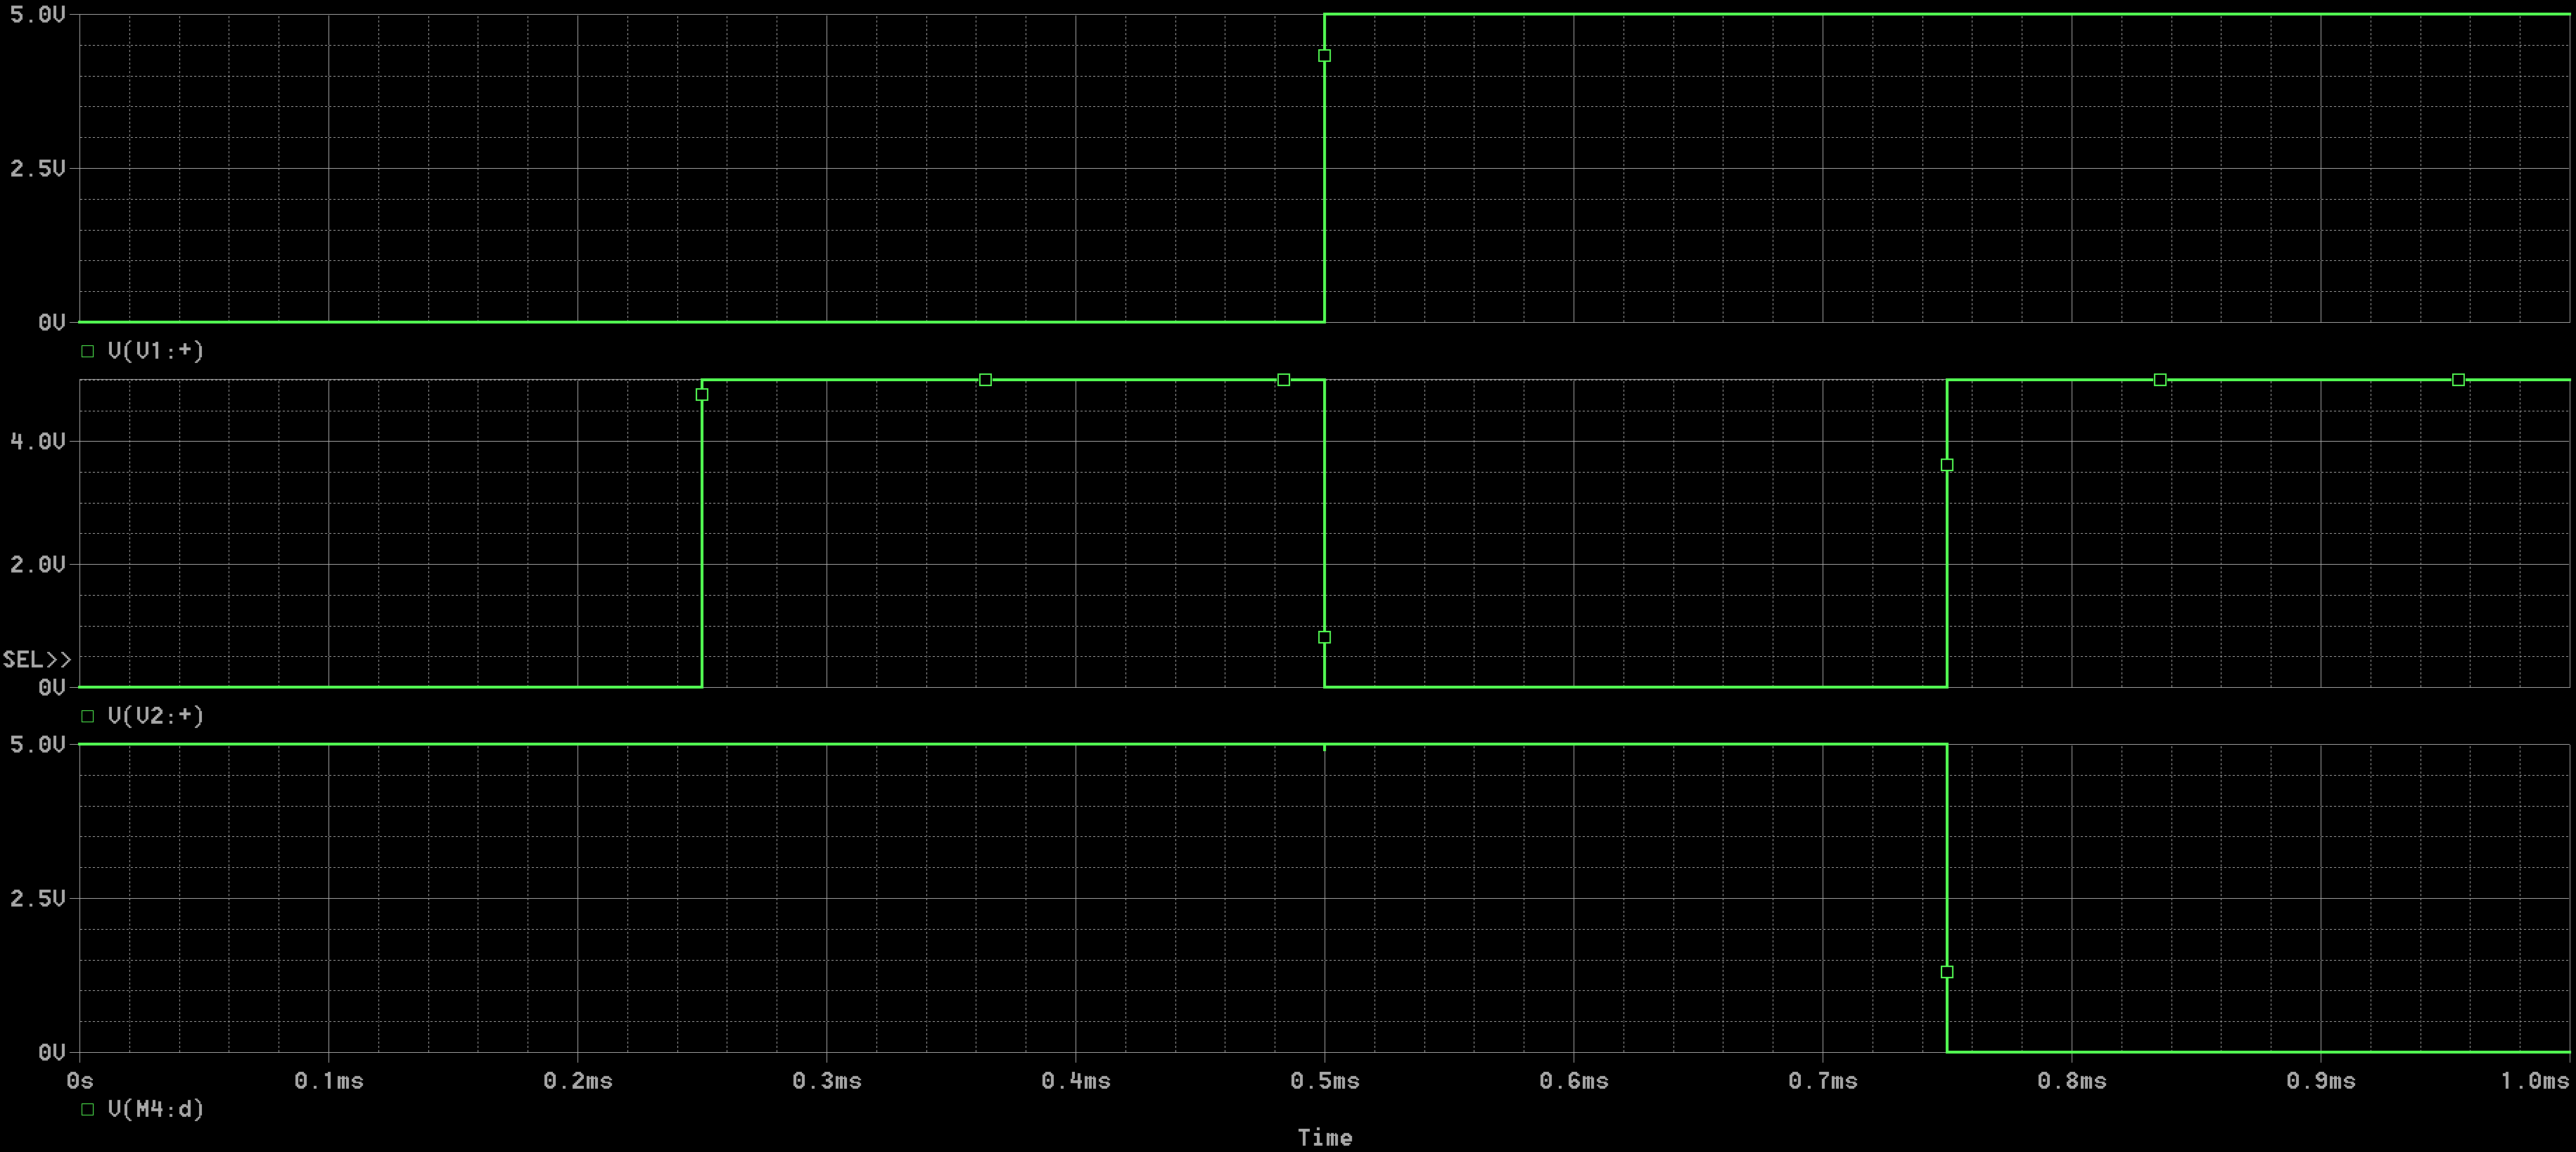
\includegraphics[scale=0.20]{../images/nand_transient_output.PNG}
	\caption{Simulated NAND Circuit Behavior}
	\label{fig:nand_sim}
\end{figure}

\FloatBarrier

The top plot shows $V_1$, which is a input square wave ($0 - 5$\si{\volt}) with a $1$\si{\kilo\hertz} frequency.
The middle plot shows $V_2$, which is a input square wave ($0 - 5$\si{\volt}) with a $2$\si{\kilo\hertz} frequency.
Lastly, the bottom plot shows the output waveform of the two-input NAND circuit.
Figure \ref{fig:nand_sim} effectively shows that the behavior of the circuit does match the truth table in Figure \ref{\tab:logic_nand}.
